\documentclass[12pt,a4paper]{jsarticle}
\usepackage[dvipdfmx]{graphicx}
\usepackage[dvipdfmx]{color}
\usepackage{url}
\usepackage{listings,jlisting}
% to use japanese correctly, install jlistings.
\lstset{
  basicstyle={\ttfamily},
  identifierstyle={},
  commentstyle={\color{red}},
  keywordstyle={\bfseries\color{cyan}},
  ndkeywordstyle={},
  stringstyle={\color{blue}},
  frame={tb},
  breaklines=true,
  numbers=left,
  numberstyle={},
  stepnumber=1,
  numbersep=1zw,
  xrightmargin=0zw,
  xleftmargin=3zw,
  lineskip=0.5ex
}
\lstdefinestyle{customCsh}{
  language={csh},
  numbers=none,
}
\lstdefinestyle{customRuby}{
  language={ruby},
  numbers=left,
}
\lstdefinestyle{customTex}{
  language={tex},
  numbers=none,
}
\lstdefinestyle{customJava}{
  language={java},
  numbers=left,
}
\begin{document}
\title{卒業論文\\
\vspace{4cm} 三面図を利用した粒界原子配列の視覚化}
\author{ 関西学院大学 理工学部 情報科学科\\\\1549 成田 大樹}
\date{\vspace{3cm} 2017年  3月\\
\vspace{3cm} 指導教員  西谷 滋人 教授}
\maketitle
\setcounter{tocdepth}{4}
\tableofcontents

%\verb|{{toc}}|
%\verb|概要(boundary_narita_summary)|

\include{introduction}

\section{ソフト開発の手法}
本研究で開発するソフト"viewer"は,小傾角粒界の原子モデルの配列を2次元で描画する.
viewerは,VASPの入出力で採用されているPOSCAR形式のファイルを読み込み,原子配列をSVGで出力する.
原子配列のSVG表示は,2次元画像描画ライブラリ"rcairo"を用いて作成していく.
それぞれについて,採用したツールや検討した内容について詳述する.

\subsection{一般的な原子モデルソフトとの比較}
結晶描画が可能なソフトとして,"Medea"および"VESTA"がある.
これらは結晶構造や電子・核密度等のデータを読み込んで結晶の形を三次元で可視化できるプログラムである\cite{vesta}.
手作業で結晶構造の視点を自由に変えることで.原子配置,並びに構造全体を視覚的に把握することができる.
図にはVESTAの画面から切り出した原子配置モデルの一例を示している.
3次元に投影することによって得られた図形である.
VESTAの使用には以下の難点があった.

\begin{itemize}
\item 三次元で原子配列を表示するため,各層の原子位置が把握しづらい
\item 色分けするための層を手動でおこなうため,指定した範囲の正確さに欠け,作業に手間がかかる
\end{itemize}
\begin{figure}[htbp]\begin{center}
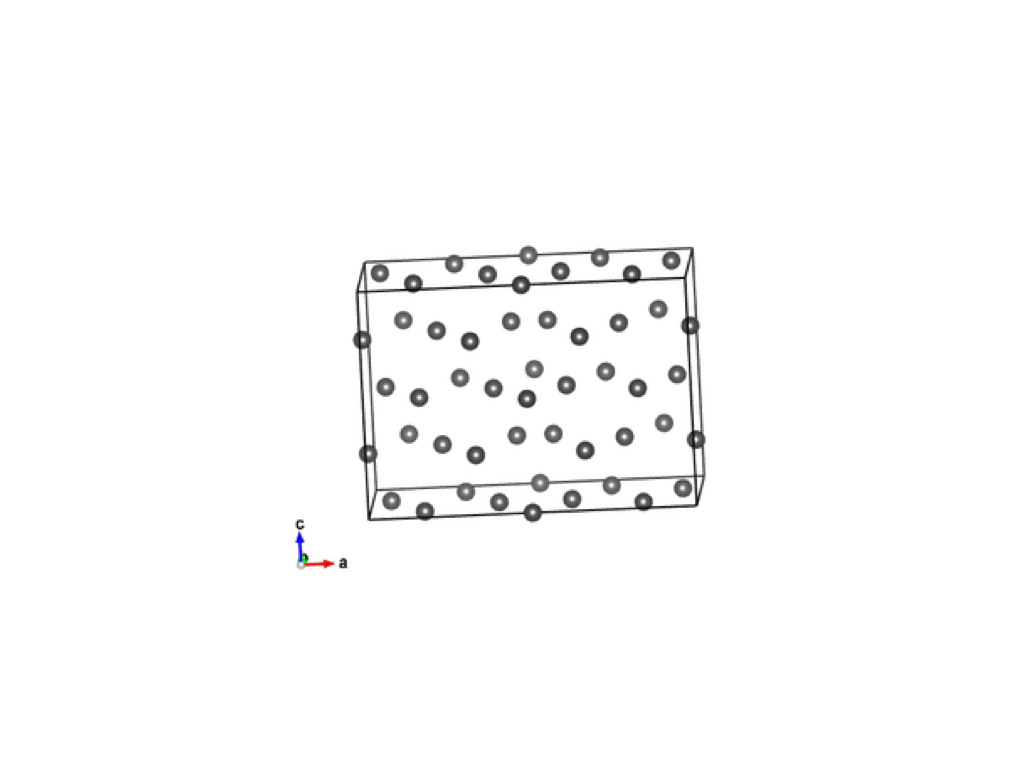
\includegraphics[width=10cm,bb= 0 0 737 553]{../figs/./boundary_narita.006.jpeg}
\caption{VESTAで描画したPOSCAR\_2223の原子配置.}
\label{default}\end{center}\end{figure}
これまでの原子配列の構造は,結晶構造描画ソフトVESTAを使用して確認してきたが.三面図を使用して表示することにより,図のように,各面から原子の配置を直感的かつ簡易に確認できるようになる.

\begin{figure}[htbp]\begin{center}
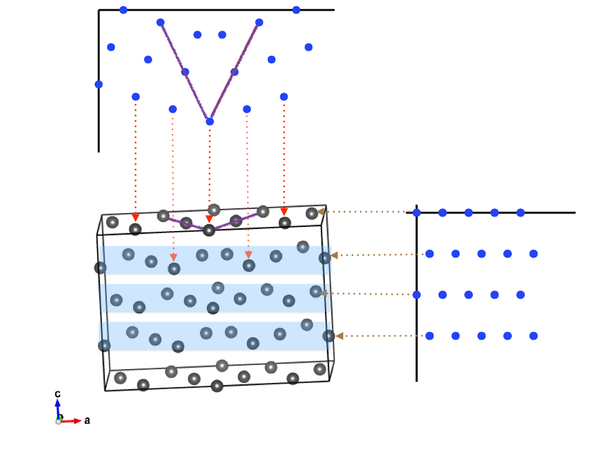
\includegraphics[width=10cm,bb= 0 0 737 553]{../figs/./boundary_narita.007.jpeg}
\caption{vestaの投影図を2次元化した図}
\label{default}\end{center}\end{figure}
\subsection{MVCモデルの概要と利点}
ソフト開発は作業の分業化が容易であるMVCモデルで作成していく.
MVCモデルは,ソフトウェアの設計モデルの一つであり,アプリケーションの開発において取られている手法である.
MVCモデルは三要素で構成されており,データの処理を担う"Model",処理結果を画面に表示する"View",入力情報の受け取って処理機能を制御する"Controller"で設計されている.各々の機能が直交化されているため,開発作業を分業化しやすく,相互の仕様変更による影響を受けずに開発を進めることが出来る\cite{mvc}.
この利点をもとに,原子配列の結果を画面表示する機能構築に特化した開発をおこなう.

\begin{figure}[htbp]\begin{center}
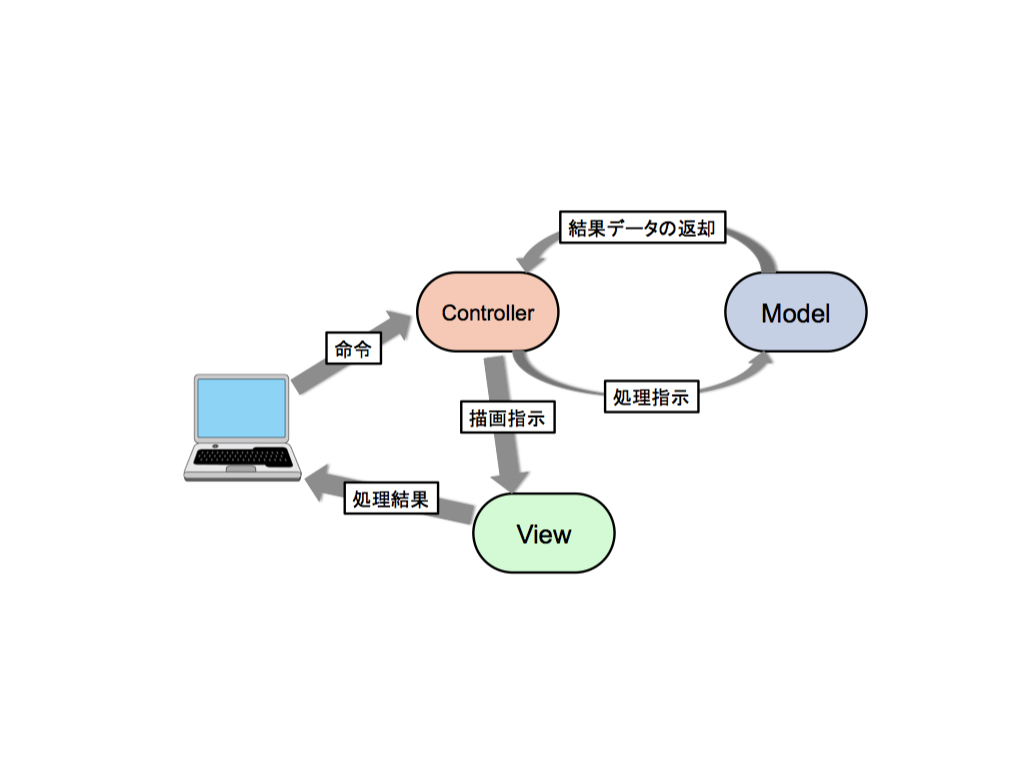
\includegraphics[width=10cm,bb= 0 0 737 553]{../figs/./boundary_narita.005.jpeg}
\caption{MVSモデルによるviewerの位置.}
\label{default}\end{center}\end{figure}
\subsection{SVG表示の特徴}
SVGは,XMLを基盤とする2次元画像記述言語であり.イラストレーターで扱うベクターデータである\cite{svg}.SVGで表示することで,以下のような利点がある.

\begin{itemize}
\item ベクタ形式で画像を表示するため,曲線や文字の拡大・縮小しても画質が劣化せずに,解像度に応じた出力結果を得ることが出来る.
\item スタイルシートを切り替えることで,特殊な環境下においても目的に応じたグラフィック描画を出力することが可能である
\item テキストデータであるため,テキストエディタやxmlプロセッサを介したファイルの編集が可能である.
\end{itemize}
\subsection{rcairoを使用する利点}
rcairoは,Ruby言語でベクタ形式の2次元描画を容易に実現できるライブラリのことである.このライブラリは,描画コンテキストを用いたAPIであるため,描画するためのコードを短く簡潔に作成することが出来る.また.複数の出力をサポートすることができるため,出力先のフォーマットに影響されずに描画処理をおこなうことが可能である\cite{cairo}.



\section{ソフトの構成}
本研究で開発したソフトは,多数の関数で構成されている.
ここからは,各関数を機能ごとに詳述する.

\subsection{外部データの読み込み部}
\subsubsection{read\_pos}\begin{lstlisting}[style=customRuby,basicstyle={\scriptsize\ttfamily}]
def read_pos(lines, init_line=8)
  lattice, atom, poscar = [],[],[]
  lines[2..4].each{|line| lattice << line.scanf("%f %f %f\n")  }
  lines[init_line..lines.length+1].each{|line| atom << line.scanf("%f %f %f\n") }

  atom.each{|i_atom|
    pos=[0.0,0.0,0.0,0.0]
    i_atom.each_with_index{|atom_j,j|
      lx,ly,lz=lattice[j]
      pos[0] += atom_j*lx
      pos[1] += atom_j*ly
      pos[2] += atom_j*lz
    }
    poscar << pos
  }
  return poscar
end
\end{lstlisting}
関数read\_posは,外部データをARGVで読み込んでいるファイルlinesを受け取って.配列に格納する機能を果たしている.
コードの3行目では,linesの2行目から4行目の値を読み込んで配列lattticeに格納しており,コードの4行目では,lines内の8行目から最後の行までの座標を読み込んで配列atomsに格納している.
6行目からは,配列atomsをeach文で繰り返し演算をおこない,その中で配列lattice内に格納された各座標をlx,ly,lzと定義している.
定義した格子の各座標と原子の各座標との積をとることで原子配列の座標をもとめ,その値を配列poscarに格納している.

原子座標ファイルPOSCAR\_2223において,配列poscarに格納された原子座標を以下の実行結果で示す.
各括弧内の数値は,左から順にx座標,y座標,z座標を表している.
\begin{lstlisting}[style=,basicstyle={\scriptsize\ttfamily}]
% ruby viewer.rb POSCAR_2223 POSCAR_2223_4

[5.75101295815, 0.0, 0.0]
[7.668017277916733, 0.6390014395849836, 2.020699977875]
[3.834008638383265, 0.6390014395849836, 2.020699977875]
[7.029015837611088, 2.556005758968566, 0.0]
[4.473010078688911, 2.556005758968566, 0.0]
[5.75101295815, 0.0, 4.04139995575]
[7.668017277916733, 0.6390014395849836, 6.062099933625]
[3.834008638383265, 0.6390014395849836, 6.062099933625]
[7.029015837611088, 2.556005758968566, 4.04139995575]
[4.473010078688911, 2.556005758968566, 4.04139995575]
[6.390014398455645, 4.473010078352149, 2.020699977875]
[5.112011517844354, 4.473010078352149, 2.020699977875]
[6.390014398455645, 4.473010078352149, 6.062099933625]
[5.112011517844354, 4.473010078352149, 6.062099933625]
[9.585021596533265, 1.2780028797985992, 0.0]
[1.917004319766734, 1.2780028797985992, 0.0]
[8.946020157377822, 3.1950071991821813, 2.020699977875]
[2.556005758922177, 3.1950071991821813, 2.020699977875]
[0.0, 1.9170043193835826, 2.020699977875]
[10.863024475994353, 3.8340086387671652, 0.0]
[0.6390014403056455, 3.8340086387671652, 0.0]
[9.585021596533265, 1.2780028797985992, 4.04139995575]
[1.917004319766734, 1.2780028797985992, 4.04139995575]
[8.946020157377822, 3.1950071991821813, 6.062099933625]
[2.556005758922177, 3.1950071991821813, 6.062099933625]
[0.0, 1.9170043193835826, 6.062099933625]
[10.863024475994353, 3.8340086387671652, 4.04139995575]
[0.6390014403056455, 3.8340086387671652, 4.04139995575]
[8.307018717072177, 5.112011518565764, 0.0]
[3.1950071992278226, 5.112011518565764, 0.0]
[10.22402303683891, 5.751012958150748, 2.020699977875]
[1.2780028794610885, 5.751012958150748, 2.020699977875]
[8.307018717072177, 5.112011518565764, 4.04139995575]
[3.1950071992278226, 5.112011518565764, 4.04139995575]
[10.22402303683891, 5.751012958150748, 6.062099933625]
[1.2780028794610885, 5.751012958150748, 6.062099933625]
\end{lstlisting}
\subsection{原子座標の計算部}
\subsubsection{identical\_atoms}\begin{lstlisting}[style=customRuby,basicstyle={\scriptsize\ttfamily}]
def identical_atom(i_atom,j_atom)
  dist=0.0
  3.times{|i| dist += (i_atom[i]-j_atom[i])**2  }
  return true if Math.sqrt(dist)<0.5
  return false
end
\end{lstlisting}
関数identical\_atomsは,読み込んで計算した2つのPOSCARファイルに含まれる各々の原子座標の距離を求め,ある値を基準に大小比較をおこなう判定をしている.
コードの3行目で,ファイル内のある原子i\_atomともう片方のファイル内にある原子j\_atomの各座標の値を差分し,その値を2乗して加えることで原子間の距離を求めている.
その距離の値が,0.5より小さい値ならばtrue,そうでなければfalseと判定して返している.

\subsubsection{mk\_deleted\_atom}\begin{lstlisting}[style=customRuby,basicstyle={\scriptsize\ttfamily}]
def mk_deleted_atom
  mark=[]
  j_max = $pos_after.length
  $pos_before.each_with_index{|i_atom,i|
    update_num=0
    $pos_after.each_with_index{|j_atom,j|
      break if identical_atom(i_atom,j_atom)
      update_num = j
    }
    mark << $pos_before[i] if update_num==(j_max-1)
  }
  return mark
end
\end{lstlisting}
関数mk\_deleted\_atomは,原子削除をおこなう前後のPOSCARファイルを比較して削除された原子のみを別の配列に格納する機能を果たしている.
具体的に,コードの5行目で更新するための値update\_numを0と定め,2つのPOSCARファイルを演算しながら,原子間の距離を求める関数identical\_atomでtrueとして返されたものを配列markへ格納している.
POSCAR\_2223において,配列markに格納された原子座標を以下の実行結果で示す.
\begin{lstlisting}[style=,basicstyle={\scriptsize\ttfamily}]
% ruby viewer.rb POSCAR_2223 POSCAR_2223_4
[[6.390014398455645, 4.473010078352149, 2.020699977875, 0.0] 
[5.112011517844354, 4.473010078352149, 6.062099933625, 0.0] 
[10.863024475994353, 3.8340086387671652, 0.0, 0.0]
 [0.6390014403056455, 3.8340086387671652, 0.0, 0.0] 
[10.863024475994353, 3.8340086387671652, 4.04139995575, 0.0]]
\end{lstlisting}
\subsection{粒界原子の描画部}
\subsubsection{draw\_backcolor, draw\_axes}\begin{lstlisting}[style=customRuby,basicstyle={\scriptsize\ttfamily}]
def draw_backcolor
  $context.set_source_rgb(0.8, 0.8, 0.8)
  $context.rectangle(0, 0, $width, $height)
  $context.fill
end

def draw_axes
  $context.set_source_rgb(0, 0, 0)
  [[0,1],[1,0]].each{|line|
    x,y=line[0],line[1]
    [[0,0],[$cx,0],[0,$cy]].each{|c_x,c_y|
      $context.move_to($mv+c_x,$mv+c_y)
      $context.line_to($mv+c_x+x*$scale,$mv+c_y+y*$scale)
      $context.stroke
    }
  }
end
\end{lstlisting}
関数draw\_backcolorは,原子配列の背景を描画しており,原子配列を表示する画面のサイズを明確にするために挿入されている.
また,関数draw\_axesは,原子配列における縦軸と横軸を描画しており,コードの11行目にて3つ平面に必要な軸をまとめて出力できるようにしている.

\subsubsection{open\_circle}\begin{lstlisting}[style=customRuby,basicstyle={\scriptsize\ttfamily}]
def open_circle
  z_layer=[]
  layer_max, layer_min = $pos_max[2], 0.0
  bound=(layer_max - layer_min )/($denominator-1)
  num,j = layer_min, 0
  $diff = 0.15
  while num <= layer_max do
    z_layer[j] = num
    num += bound
    j += 1
  end
  return z_layer
end
\end{lstlisting}
関数open\_circleは,白抜きする層の座標を計算して配列に格納している.
コードの3行目に記述されたlayer\_maxは,関数find\_maxで得た原子のz座標の最大値を取っており,layer\_minはz座標の最小値として初期値0を与えている.
その直後に挿入されているboundは,各層の倍数値を取っている.
この倍数値は,z座標の最大値と最小値の差をとり,差分した数値を関数main\_drawで読み込んだ分母値denominatorで割ることにより値を得ている.
コードの7行目では,layer\_minからlayer\_maxまでの範囲で倍数値boundを加算させていき,加えていった各数値を配列z\_layerに格納している.
また,コード内に挿入されているdiffは,関数draw\_each\_planeにて白抜きする原子座標の近似値をさす.

\subsubsection{pos\_y}\begin{lstlisting}[style=customRuby,basicstyle={\scriptsize\ttfamily}]
def pos_y(pos, c_y, index, select)
  dy = select == 0 ? pos[index] : $pos_max[index]-pos[index]
  return $mv+c_y+$adjust*dy
end
\end{lstlisting}
関数pos\_yでは,x−y平面のy軸を逆転させる計算をおこない.描画する原子のy座標を返している.
具体的に,関数draw\_each\_planeの中のselで,描画する平面を識別した結果をもらい,x−y平面ならば,関数find\_maxにより得たy座標の最大値から各y座標を差分し,その値をdyへ与えている.
x−y平面以外の平面ならば,最大値からの差分を取らずにそのままの値を返している.

\subsubsection{draw\_each\_plane}\begin{lstlisting}[style=customRuby,basicstyle={\scriptsize\ttfamily}]
def draw_each_plane(ind_1,ind_2,c_x,c_y)
  rr = 2
  sel = (ind_1==0 and ind_2==1)? 1 : 0
  [[$deleted_atoms,[1,0,0],rr*1.3],[$pos_after,[0,0,1],rr]].each{|atoms_color|
    $context.set_source_rgb(atoms_color[1])
    radius = atoms_color[2]
    atoms_color[0].each{|pos|
      if $numerator == 0 then
        $context.circle($mv+c_x+$adjust*pos[ind_1],pos_y(pos,c_y,ind_2,sel), radius)
        $context.fill
      else
        if pos[2] < open_circle[$numerator-1]+$diff and open_circle[$numerator-1] - $diff < pos[2] then
          $context.circle($mv+c_x+$adjust*pos[ind_1],pos_y(pos,c_y,ind_2,sel), radius*1.7)
          $context.stroke
          $context.set_line_width(0.5)
        else
          $context.circle($mv+c_x+$adjust*pos[ind_1],pos_y(pos,c_y,ind_2,sel), radius)
          $context.fill
        end
      end
    }
  }

  if $pos_before.size==$pos_after.size
    $context.set_source_rgb(0, 0.8, 0)
    (0..$pos_before.length-1).each{|i|
      $context.move_to($mv+c_x+$adjust*$pos_before[i][ind_1],pos_y($pos_before[i],c_y,ind_2,sel))
      $context.line_to($mv+c_x+$adjust*$pos_after[i][ind_1],pos_y($pos_after[i],c_y,ind_2,sel))
      $context.stroke
    }
  end
end
\end{lstlisting}
関数draw\_each\_planeでは,描画する原子の位置,色,大きさを決定し,白抜き処理の判定をおこなっている.
コードの2行目にある値rrは,原子の半径値を示している.
4行目から,atoms\_colorの配列を組んで削除の有無により原子の色と大きさを変えて描画するようにしている.
また,8行目からは,原子の白抜き処理を判定している.具体的に,分子値numeratorが0であるかを判定し,trueならば白抜きなしの原子配列を描画する.
分子値numeratorが0でない,すなわち指定した層の値がnumeratorに入力されているのならば,関数open\_circleで各層の値を格納しているz\_layerの配列番号を指定し,近似値diffで範囲を求め,指定した層の白抜き処理をおこなう.
さらに,24行目からは,読み込んだ2つの原子配列ファイルPOSCARのデータサイズを比較している.同じサイズであるならば,2つのファイルにおける各原子間の距離を線で表示するようにしている.

\subsubsection{draw\_atoms}\begin{lstlisting}[style=customRuby,basicstyle={\scriptsize\ttfamily}]
def draw_atoms
  draw_each_plane(0,1,0,0)    
  draw_each_plane(0,2,0,$cy)   
  draw_each_plane(1,2,$cx,$cy) 
end
\end{lstlisting}
関数draw\_atomsでは,関数draw\_each\_planeで決定された原子配列を三面図の規定位置にそれぞれ描画するようにしている.
具体的に,x−y平面を平面図として第二象限,x−z平面を正面図として第三象限,y−z平面を側面図として第四象限に出力させている.

\subsubsection{find\_max}\begin{lstlisting}[style=customRuby,basicstyle={\scriptsize\ttfamily}]
def find_max(pos)
  max = [0,0,0]
  [0,1,2].each{|ind|
    pos.length.times {|i| max[ind] = pos[i][ind] if max[ind] < pos[i][ind] }
  }
  return max
end
\end{lstlisting}
関数find\_maxは,原子の各座標の最大値を探索する機能を果たしている.
関数read\_posにて,原子のx座標,y座標,z座標をそれぞれpos[0],pos[1],pos[2]の中に格納しており,隣接する値を比較することで,各座標の最大値を探索し,配列maxに格納している.

\subsubsection{main\_draw}\begin{lstlisting}[style=customRuby,basicstyle={\scriptsize\ttfamily}]
def main_draw(file1,file2, layer, model_scale = 10)
  lines1 = File.readlines(file1)
  lines2 = File.readlines(file2)
  if layer != nil then
    tmp=layer.split('/')
    $numerator, $denominator = tmp[0].to_f,tmp[1].to_f
  else
    $numerator = 0
  end
  
  $pos_before, $pos_after = read_pos(lines1,8), read_pos(lines2,8)
  $deleted_atoms = mk_deleted_atom
  
  $pos_max=find_max($pos_before)
  $pos_max[0].ceil*10
  $width,$height = 300,200
  $cx,$cy = $width/2.0,$height/2.0
  $mv = 10
  $scale = 1000
  $adjust = $scale/($pos_max[0].ceil*model_scale)
  surface = Cairo::SVGSurface.new('view.svg', $width, $height)
  $context = Cairo::Context.new(surface)
  $context.set_line_width($line_width)
  draw_backcolor
  draw_axes
  draw_atoms
  surface.finish
end
\end{lstlisting}
関数main\_drawには,描画機能の基盤が設定されており,rcairoで描画処理の基本となるサーフェスとコンテキストを作成し,出力場所及び出力先の形式を定めている.
2,3行目のlinesには,読み込んだ各々の外部ファイルを格納しており,コードの4行目では,白抜きする層の値が入力されているかを判定している.
この判定がtrueならば,入力値を/で分別し,それぞれの数値を分子値numerator, 分母値denominatorとして与えている.
また,判定がfalseならば,numeratorに0を与えている.
11行目では,読み込んだ2つの原子配列ファイルを関数read\_posで計算し,作成した原子座標poscarをファイルごとに分類している.
具体的に,初めのファイルの方をpos\_before,他方をpos\_afterとしている.
width,及びheightは,出力するスクリーンの大きさを指定しており,18行目のmvは,出力全体を移動させるための値である.
これは,軸上に存在している原子がスクリーンから出てしまうのを防ぐために挿入されている.
その直後に挿入されているscale,adjustは,出力する軸,並びに原子の大きさである.

なお,プログラムの文末には以下のコードを記述している.
\begin{lstlisting}[style=customRuby,basicstyle={\scriptsize\ttfamily}]
model_scale = 1.0/0.12
$line_width = 1
main_draw(ARGV[0],ARGV[1], ARGV[2],model_scale)
\end{lstlisting}
model\_scale,line\_widthは,出力する画面に対して軸や原子の大きさを調整するための数値である.

\subsection{三面図による描画}
三面図は,立体を正面図,平面図,側面図の三方向からみて投影した図を展開したもので,立体の形状を2次元上で的確に表示することが出来る.
開発当初は,上面,正面,側面の配置をまったく気にせずに図(a)のように配置していた.
しかし,三方向から描く各図の位置はJIS規格で厳密に定めされており,正面図を物体の最も代表的な面と決められている\cite{ThreeViewDrawing}.
その正面図の真上に平面図,正面図の真横に側面図を描くことで三面図が作成される.
そこで,図(b)のとおり最終版では修正して配置している.

\begin{figure}[htbp]\begin{center}
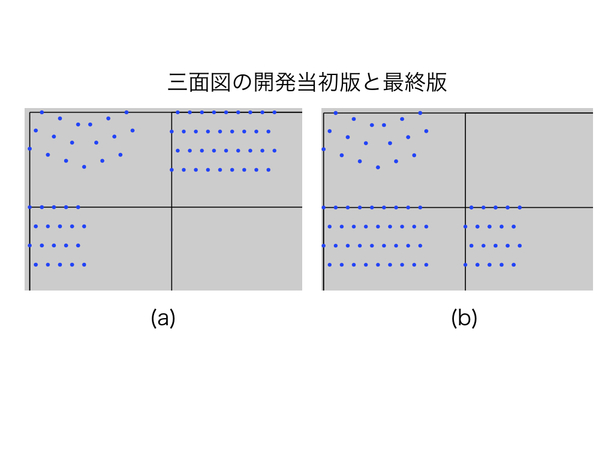
\includegraphics[width=12cm,bb= 0 0 937 753]{../figs/./boundary_narita.014.jpeg}
\caption{POSCAR\_2223を表示した三面図の(a)開発当初版と(b)最終版.}
\label{default}\end{center}\end{figure}


\section{結果と考察}
\subsection{各用途に合わせた原子配列の表示結果}
\subsubsection{削除された原子の識別表示}
原子の削除操作は,岩佐の研究で最安定の原子配列の構造を探索するために取り入れた手法である.
boundary modelerで2223などと指定して作成された原子配置では,真ん中と両端にある粒界近傍で原子位置の極端に近いペアが生成する.このままでは,高いエネルギーとなり緩和がうまく進行しない.そこで,boundary adjusterで原子の削除を行う.削除前後のPOSCARを比較して原子位置を特定する作業をVESTAなどでは手動で行うが,この削除された原子の位置を視覚的に把握しやすくするための表示法を工夫した.なお,以下のコードを入力することでsafari上に表示される.
\begin{lstlisting}[style=customCsh,basicstyle={\scriptsize\ttfamily}]
% ruby viewer.rb POSCAR_2223 POSCAR_2223_4
% open -a safari view.svg 
\end{lstlisting}
原子の削除有無を識別した三面図は,図\ref{fig:010}のように表示される.

\begin{figure}[htbp]\begin{center}
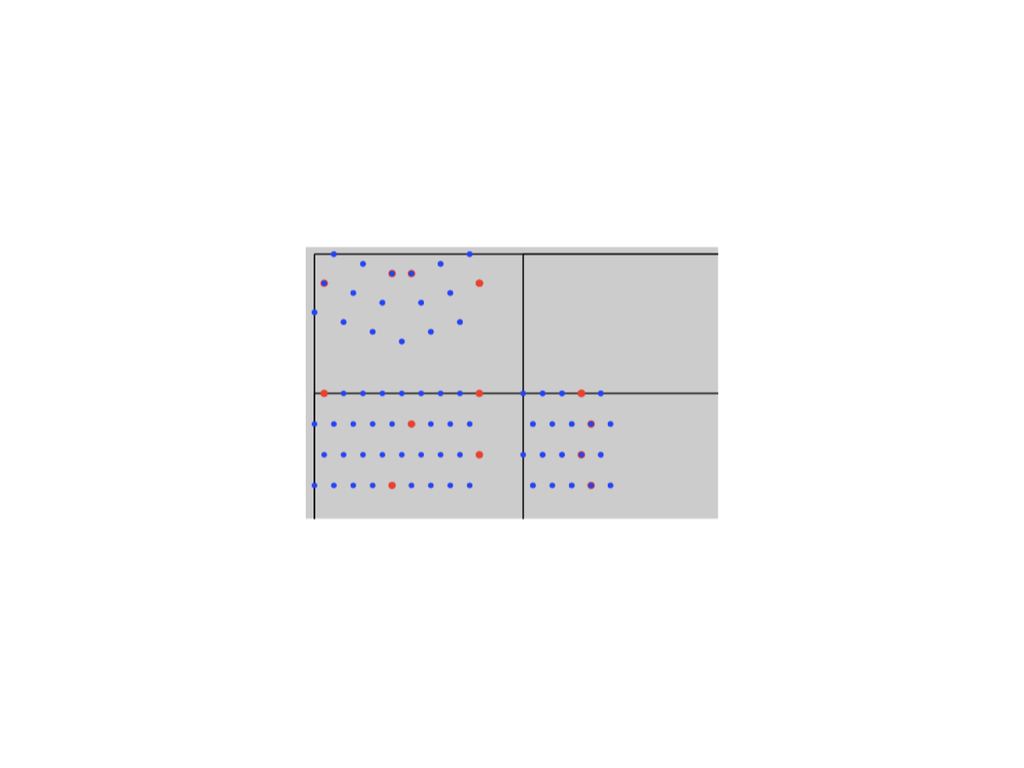
\includegraphics[width=10cm,bb= 0 0 937 753]{../figs/./boundary_narita.010.jpeg}
\caption{削除前後のPOSCARを色分けした三面図.}
\label{fig:010}
\label{default}\end{center}\end{figure}

図中の赤い丸が削除された原子に相当する.
平面図では青と赤が重なっているが,これは正面図からわかる通り,上下に重なった原子位置で削除の有無が存在するためである.
VESTAなどの汎用ソフトでは,このような操作は標準で用意されておらず,原子種を変えるなどの工夫によって表示することが必要である.
しかし,開発したviewerでは二つのPOSCARの原子位置から自動で判定するようにしている.
また,三面図で描画したことにより,削除された原子数,並びに各々の配置をすぐに把握することができた.
これは後で説明するとおり,粒界構造の確認の時に決定的なエラーに気づかせてくれた.

\subsubsection{構造緩和による原子移動の表示}
粒界原子配列の構造緩和は,最安定の原子配列を検証するために動かす前後のエネルギーを比較して原子を動作させる手法である.
原子の移動を表した図は,同様のソフトに構造緩和前後を示した2種類のファイルを入力して表示される.
\begin{lstlisting}[style=customCsh,basicstyle={\scriptsize\ttfamily}]
% ruby viewer.rb POSCAR_after POSCAR_before
% open -a safari view.svg 
\end{lstlisting}
以下の図\ref{fig:011}は,構造緩和によって移動した原子配列の三面図である.

\begin{figure}[htbp]\begin{center}
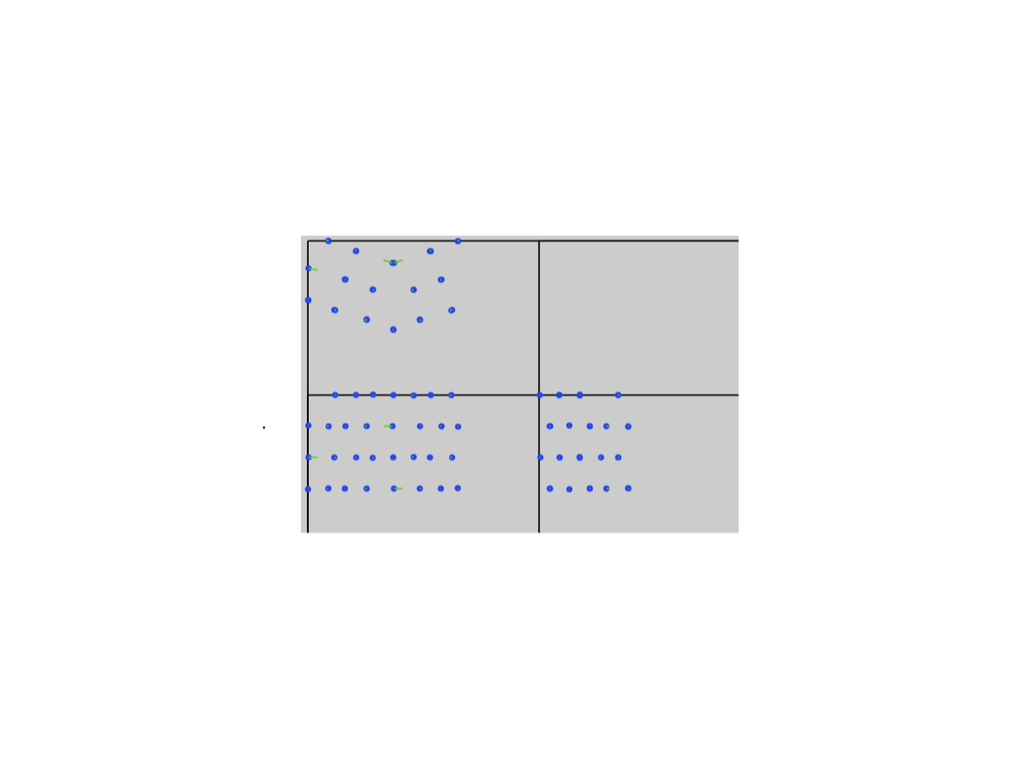
\includegraphics[width=10cm,bb= 0 0 937 753]{../figs/./boundary_narita.011.jpeg}
\caption{構造緩和前後による原子の移動を示した三面図.}
\label{fig:011}
\label{default}\end{center}\end{figure}

図中の緑線は,構造緩和をおこなう前後で各原子が移動した経路である.
この三面図はSVGで表示されているため,拡大しても解析度が落ちずに鮮明に描画することができ,原子の移動変化をより細かく見ることができる.
その結果,原子の正確な移動位置,並びに第一原理計算ソフトVASPによる系全体のエネルギーを計算する際の構造緩和に過ちが生じていないかを
容易に判断できるようになった.

\subsubsection{指定したz軸の層の白抜き表示}
POSCAR\_2223は4層の原子配列で構成されているため,原子配列を上から見た図,すなわち平面図では,原子同士が重なって配置してしまう.
したがって,指定した層の原子が平面図の中でどこに位置するのかを視覚的に確認するために原子の白抜き処理をおこなった.
白抜き処理は,読み込む2つのファイル名の後に白抜きする層の段階数を入れることで表示される.
層の段階数は上層から順に数字を割り振っており,分母が層の総数,分子が白抜きしたい層である.
以下の実行は,4層で構成されているPOSCAR\_2223の第1層目を白抜き処理する際に入力したものである.
\begin{lstlisting}[style=customCsh,basicstyle={\scriptsize\ttfamily}]
% ruby viewer.rb POSCAR_2223 POSCAR_2223_4 1/4
% open -a safari view.svg 
\end{lstlisting}
このときに表示された原子配列の三面図は.以下の図\ref{fig:012}である.

\begin{figure}[htbp]\begin{center}
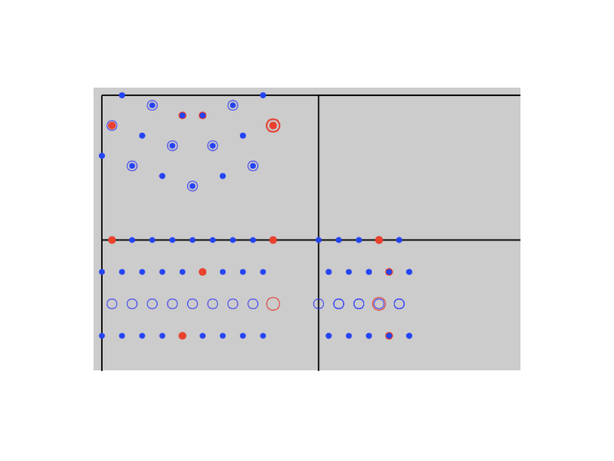
\includegraphics[width=8cm,bb= 0 0 937 753]{../figs/./boundary_narita.012.jpeg}
\caption{第一層目の原子を白抜きした三面図.}
\label{fig:012}
\label{default}\end{center}\end{figure}

この表示結果により,平面図と正面図の対応した位置が正確に判断できるだけでなく,図\ref{fig:013}のように平面図と側面図で対応した原子の位置を視覚的に判断することが可能になった.

\begin{figure}[htbp]\begin{center}
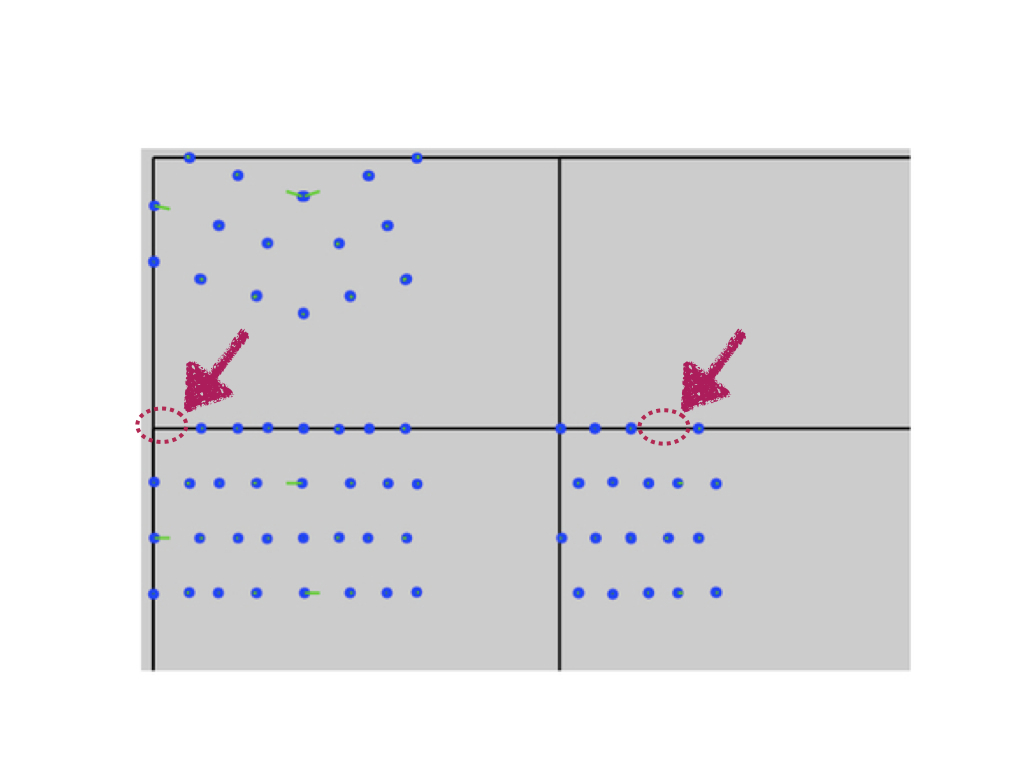
\includegraphics[width=8cm,bb= 0 0 937 753]{../figs/./boundary_narita.013.jpeg}
\caption{各図面の配置に対応していることを明示した図.}
\label{fig:013}
\label{default}\end{center}\end{figure}

なお,読み込む2つのファイル名の後に数値を入力しない,若しくは分子に0の値を入力することにより,白抜きなしの三面図を表示することが可能である.
\subsection{原子構造の改善点}
viewerによって三方向の視点で原子配列を表示した結果,構造緩和をおこなうためのPOSCARファイルに原子が一つ不足していることが分かった.
不足していた原子の位置は,図\ref{fig:014}の赤枠部分である.

\begin{figure}[htbp]\begin{center}
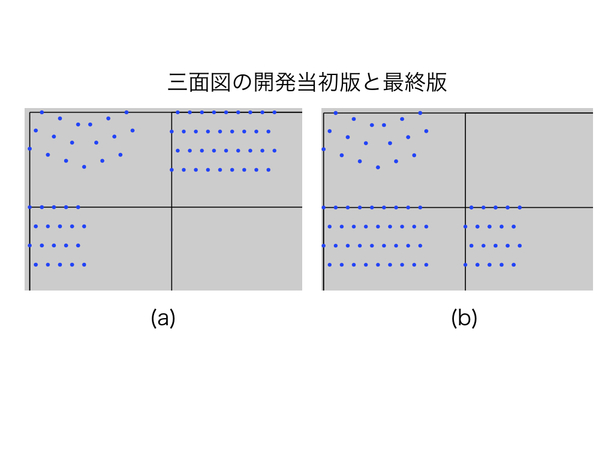
\includegraphics[width=8cm,bb= 0 0 937 753]{../figs/./boundary_narita.014.jpeg}
\caption{不足した原子を三面図で明示した図.}
\label{fig:014}
\label{default}\end{center}\end{figure}
この表示が,viewerによる計算,描画の誤りでないかを検証する必要があるため,ファイルPOSCAR\_afterの原子配列をVESTAで三次元化して確認をおこなった.
以下の図\ref{fig:015}は,構造緩和後のPOSCARファイルをVESTAで表示したものてある.

\begin{figure}[htbp]\begin{center}
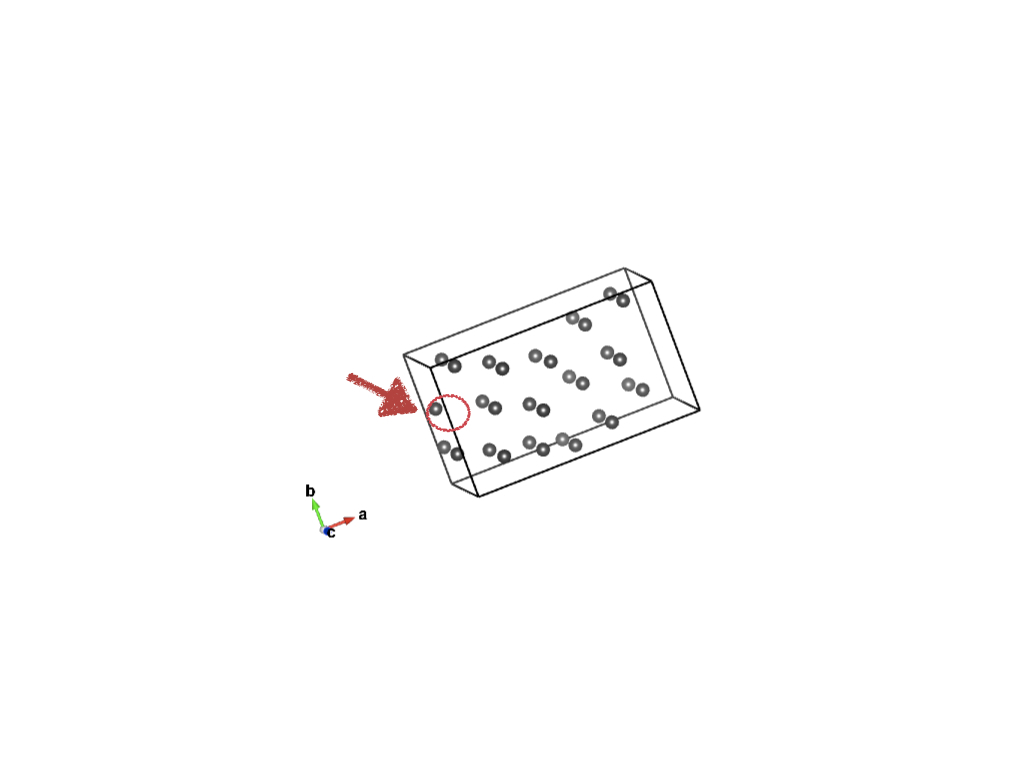
\includegraphics[width=11cm,bb= 0 0 937 753]{../figs/./boundary_narita.015.jpeg}
\caption{不足した原子をVESTAで視覚的に検証した図.}
\label{fig:015}
\label{default}\end{center}\end{figure}
その結果,図のように各々の位置で対応する原子がある中で,赤枠で括った部分には対応した原子が存在していないのが分かった.
したがって,三面図による不足した原子の発見はソフト内の過ちではないことが視覚的に確認できた.

\subsection{考察と今後の課題}
三面図を利用して原子配列を表示したことで,構造緩和をおこなう際に使用したPOSCARファイルに過ちがあったことに気づいた.
これは,今までの原子配列が結晶構造描画ソフト"VESTA"による三次元表示であり,原子の細かい位置が確認できず,原子が不足していることを認識できなかったためである.
したがって,粒界原子配列の構造緩和をおこなう計算を見直す必要がある.
また,本研究ではPOSCAR\_2223を基準として様々な描画を出力できるソフトを開発したが,より大きな粒界原子配列を視覚的に検証できるように改良していかなければならない.
さらに,三面図の配置では,正面図を物体の最も代表的な面と規定されているが,原子配列の表示で最も重要な面は,上から見た図,すなわち平面図であることが開発後に分かった.
したがって,今後は三面図の配置構成を図\ref{fig:016}のように変更して視覚的検証をおこなっていく.

\begin{figure}[htbp]\begin{center}
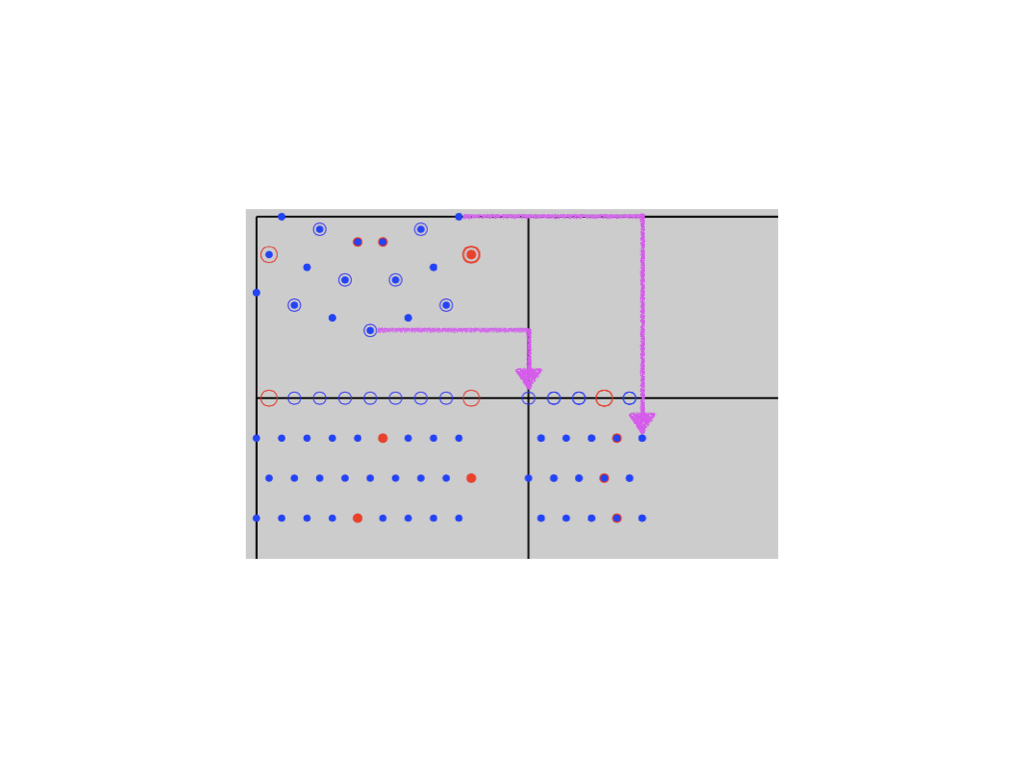
\includegraphics[width=12cm,bb= 0 0 937 753]{../figs/./boundary_narita.016.jpeg}
\caption{正面図と平面図の配置を変更した図.}
\label{fig:016}
\label{default}\end{center}\end{figure}

\section{総括}
 本研究は,最安定の構造をとるためにおこなう原子の削除操作,及び構造緩和を視覚的に,且つ容易に把握できるソフトを開発することが目的であった.
作成したソフトは,rcairoを用いて2次元で小傾角粒界の原子配列を描画し,SVG形式の三面図で表示するようにした.\\
 開発を進めた結果,様々な用途に合わせて原子配列を表示することが可能となった.
まず,削除操作を表した原子配列の表示では,削除の有無により原子の色と大きさを変えて描画したことで,削除された原子の個数,並びに各位置を視覚的に把握することができた.
また,構造緩和による原子移動の表示では,構造緩和前後で原子が移動した経路を示すことができ,構造緩和に過ちが生じていないかを容易に確認できるようになった.
さらに,指定したz軸の層の原子を白抜きする機能を追加したことで,上面から見た各層の原子位置を正確に把握できるようになった.
三面図による描画,並びにVESTAによる視覚的検証の結果として,構造緩和前後の原子座標を格納したPOSCARファイル内に原子が一つ不足していることが発見できた.

 今後は,粒界原子配列の構造緩和をおこなう計算を見直す研究を進めていく必要がある.
さらに,本研究では,一つの原子配列ファイルをもとに様々な表示ができるソフトを開発したが,このソフトをより大きな粒界原子配列を表示できる機能へ改良していかなければならない.


\section{参考文献}
\begin{thebibliography}{9}
\bibitem{Murakami} VASPによる粒界エネルギーの第一原理計算, 村上成那 (関西学院大学 理工学部研究科情報科学専 攻 修士論文 2014)

\bibitem{Yahata} 小傾角粒界粒子シミュレーションの原子ポテンシャル依存性, 八幡裕也 (関西学院大学 理工学部研究科情報科学専 攻 修士論文 2015)

\bibitem{Iwasa} 原子削除操作を加えた対称傾角粒界のエネルギー計算, 岩佐恭佑 (関西学院大学 理工学部研究科情報科 学士論文 2016)

\bibitem{vesta} VESTA, Koichi Momma(2004-2017), JP-Minerals. %\verb|http://jp-minerals.org/vesta/jp/| 

\bibitem{mvc} MVC(Model-View-Controller)を理解する, CakePHP. %\verb|https://book.cakephp.org/2.0/ja/cakephp-overview/understanding-model-view-controller.html| 

\bibitem{svg} SVG入門, 新山祐介, コンピュータサイエンス入門 by 新山祐介. %\verb|https://euske.github.io/euskecs/lec_svg/index.html| 

\bibitem{cairo} cairo:2次元画像描画ライブラリ, 須藤功平, Rubyist Magazine-るびま Vol.54 (2016-08). %\verb|http://magazine.rubyist.net/?0019-cairo| 

\bibitem{views} 三面図(機械設計のための基礎製図), 独立行政法人 海上技術安全研究所, NMRI. %\verb|https://www.nmri.go.jp/eng/khirata/mechdesign/ch04/ch04.html|
\end{thebibliography}


\end{document}
